% Group 13 project plan (design documentation), due Fri 27.11.2026 23:59 on Moodle.
% Built on the course template (materials/project-template/main.tex): same document class and
% the same section names, so this file can grow into the final report.
% Compile on Overleaf: upload this file, architecture.pdf (or .png) and press Recompile.
\documentclass{article}
\usepackage[T1]{fontenc}
\usepackage[utf8]{inputenc}
\usepackage{lmodern}
\usepackage[margin=2.3cm]{geometry}
\usepackage{graphicx}
\usepackage{booktabs}
\usepackage{tabularx}
\usepackage{array}
\usepackage{float}
\usepackage[hidelinks]{hyperref}

\newcolumntype{L}{>{\raggedright\arraybackslash}X}
\renewcommand{\arraystretch}{1.18}
\newcommand{\dps}{\,$^\circ$/s}

\title{Edge-ML Gesture Controller:\\ On-Device Gesture Recognition and MQTT Control with the Pico W\\[4pt]
\large Project plan, group 13}
\author{Syed Amin Al Mahim, Duong Vo, Yumish Niroula}
\date{27 November 2026}

\begin{document}

\maketitle

\noindent\textit{Keywords:} Raspberry Pi Pico W, IMU, gesture recognition, decision tree, edge machine learning, MQTT, InfluxDB, Grafana\\
\noindent\textit{Code:} \url{https://github.com/hasibmahim/edge-ml-gesture-controller}

\section{Introduction}

The idea is a small wearable or hand-held controller. You do a gesture with the board in your hand, the Pico W recognises it, and something happens: a lamp on another device turns on or off, the result shows on the OLED, and the event is stored and shown on a dashboard. Gesture input makes sense when your hands are busy or dirty, for example in a lab, a workshop or a kitchen, or for someone who cannot easily use small buttons.

The more interesting part for us is where the recognition runs. A wearable could just stream its raw sensor data to a server and let the server classify it. That is simple, but it sends a lot of data and it stops working when the network goes. Or the device can classify the gesture itself and only send the result. So, our project question is this: \emph{for a microcontroller like the Pico W, does classifying gestures on the device instead of on a server reduce network traffic and delay enough to matter, and what does it cost in accuracy, model size and time on the device?} We build both ways with the same model and measure them against each other.

We use the TKJ HAT that our group has from the Computer Systems course. It has an ICM-42670 accelerometer and gyroscope, an OLED display, an RGB LED, a buzzer and two buttons, so we do not need extra hardware. Our HAT is already mounted on a Raspberry Pi Pico WH (a Pico W with headers) inside a hand-held case, so Wi-Fi is there and the board is held the same way every time, which helps the gesture recognition. From the pin lists, the HAT does not use the pins of the Pico W's wireless chip (GPIO 23, 24, 25 and 29), but we still have to check in MicroPython that the IMU and the OLED answer. Table~\ref{tab:req} shows which course requirements the project covers.

\begin{table}[H]
\centering
\caption{Course requirements and how the project meets them.}
\label{tab:req}
\begin{tabularx}{\textwidth}{@{}l L l@{}}
\toprule
Requirement & How we meet it & Type \\
\midrule
Sensor data collection & ICM-42670 IMU on I2C: 3-axis acceleration and 3-axis rotation at 50 Hz & required \\
Data processing on the Pico W & Motion-triggered 1.5 s windows, 40 features per window, confidence threshold and cooldown & required \\
Output control & OLED text, RGB LED colour and buzzer per gesture; a second Pico W switches its LED on and off & required \\
Wireless connectivity & MQTT over Wi-Fi (\texttt{umqtt.simple} on the Pico W, Mosquitto broker) & optional 1 \\
Edge machine learning & Decision tree trained on our own data, exported to MicroPython and run on the Pico W & optional 2 \\
Cloud integration & Node-RED stores events and measurements in InfluxDB, Grafana shows them & optional 3 \\
Security & MQTT over TLS with username and password, only if time allows & stretch \\
Mobile app & Not claimed. We have a small web page that shows the live data and switches the mode, but it is not an Android or iOS app. & -- \\
\bottomrule
\end{tabularx}
\end{table}

\section{Architecture}

Figure~\ref{fig:arch} shows the system in three layers. The blue path is edge mode and the orange path is cloud mode. Solid boxes are already written and tested on a PC; dashed boxes are still to build. Nothing has run on the real board yet.

\begin{figure}[H]
\centering
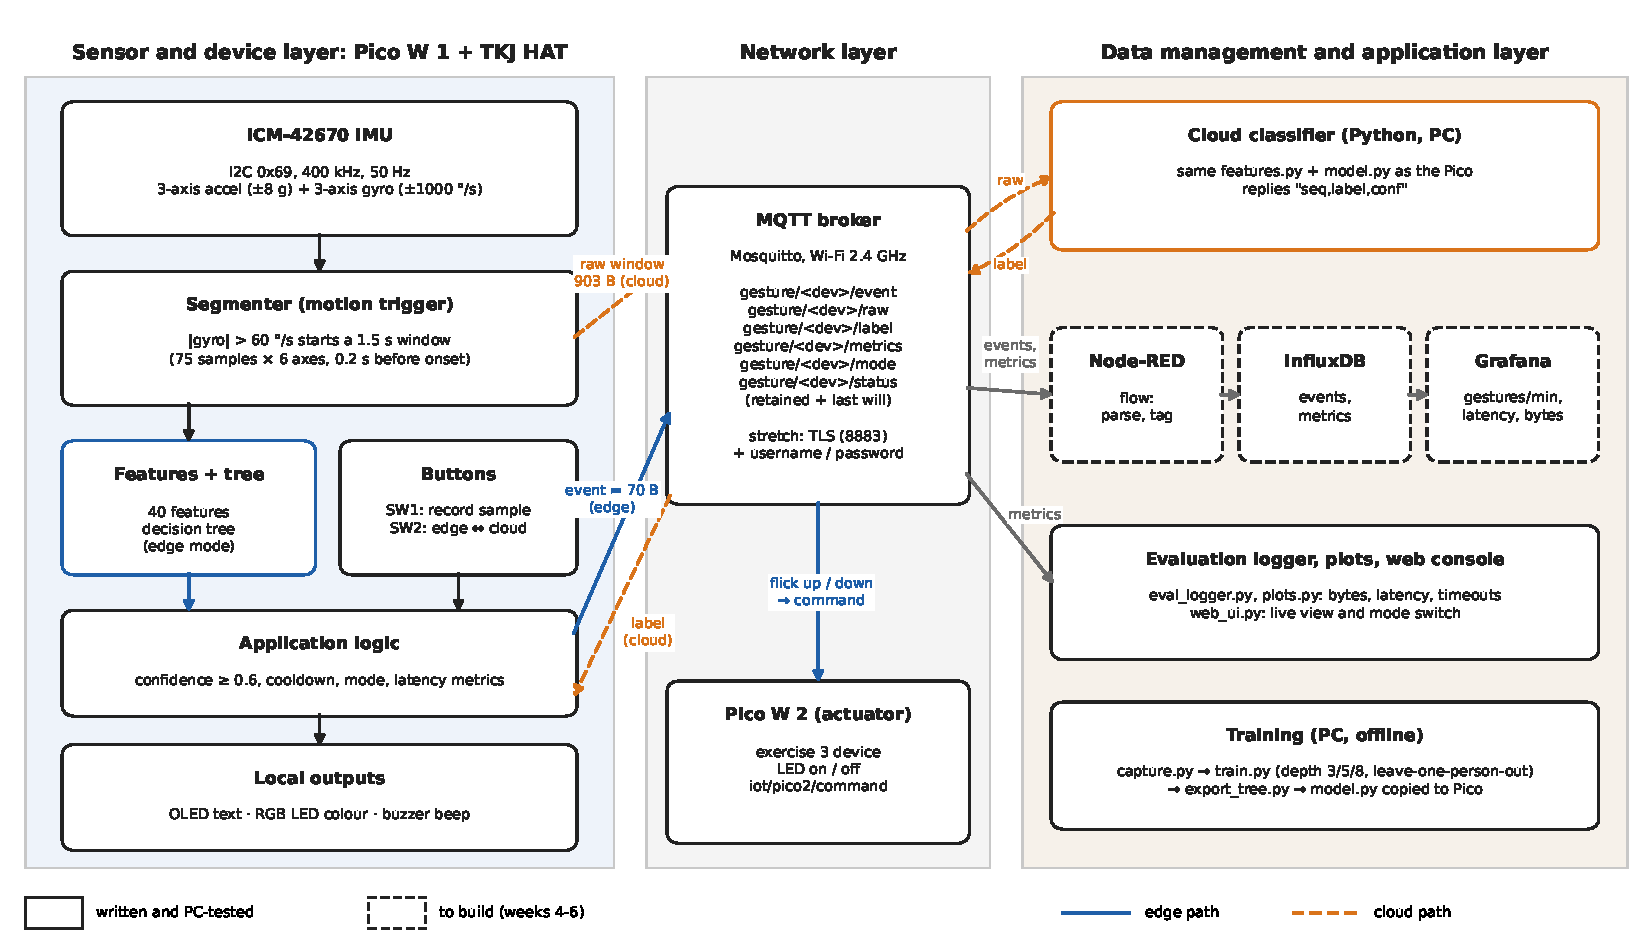
\includegraphics[width=\textwidth]{architecture}
\caption{System architecture. In edge mode the Pico W classifies the window and publishes only the result. In cloud mode it publishes the raw window, and a Python service classifies it with the same model and replies.}
\label{fig:arch}
\end{figure}

\subsection{Sensor and device layer}

The IMU is read over I2C at 400 kHz with a sampling rate of 50 Hz. We set it to $\pm$8 g and $\pm$1000\dps\ instead of the SDK default of $\pm$4 g and $\pm$250\dps, because shakes and flicks would clip at the default. A segmenter watches the rotation speed. When it goes above 60\dps\ it cuts a 1.5 s window (75 samples of 6 axes) that starts 0.2 s before the movement. In edge mode the Pico computes 40 features from the window and runs the decision tree. The application logic then checks the confidence (at least 0.6), ignores the ``idle'' class, and drives the OLED, LED and buzzer. SW2 switches between edge and cloud mode, and SW1 records labelled samples when the Pico runs the data collection program.

\subsection{Network layer}

All communication is MQTT over the 2.4 GHz Wi-Fi, with a Mosquitto broker on a laptop in the same network. Table~\ref{tab:topics} lists the topics. The status topic is retained and has a last will, so any subscriber can see whether the controller is online. The Pico W reconnects Wi-Fi and MQTT in the background, so gesture recognition and the local outputs keep running while the network is down.

\begin{table}[H]
\centering
\caption{MQTT topics (\texttt{DEV} is the device name, for example \texttt{gesture1}).}
\label{tab:topics}
\begin{tabularx}{\textwidth}{@{}l l L@{}}
\toprule
Topic & Direction & Payload \\
\midrule
\texttt{gesture/DEV/event} & Pico $\rightarrow$ & JSON: gesture, confidence, mode (about 70 bytes with the topic) \\
\texttt{gesture/DEV/raw} & Pico $\rightarrow$ & Cloud mode only. Binary: 3-byte header and 6 $\times$ 75 int16 values = 903 bytes \\
\texttt{gesture/DEV/label} & $\rightarrow$ Pico & Cloud mode only. Text: \texttt{seq,label,confidence} \\
\texttt{gesture/DEV/metrics} & Pico $\rightarrow$ & JSON per window: sequence number, mode, gesture, confidence, latency, bytes \\
\texttt{gesture/DEV/mode} & $\rightarrow$ Pico & \texttt{edge}, \texttt{cloud} or \texttt{hybrid}, to switch the mode remotely \\
\texttt{gesture/DEV/status} & Pico $\rightarrow$ & \texttt{online} / \texttt{offline}, retained, last will \\
\texttt{iot/pico2/command} & Pico $\rightarrow$ Pico 2 & \texttt{on} after flick up, \texttt{off} after flick down \\
\bottomrule
\end{tabularx}
\end{table}

\subsection{Data management and application layer}

The cloud classifier is a small Python service on the laptop. It imports the same feature code and the same exported model as the Pico, so both modes give the same answer for the same window, and the comparison is only about where the work happens. Node-RED subscribes to the event and metrics topics and writes them to InfluxDB. We plan one measurement for gestures with \texttt{device}, \texttt{mode} and \texttt{gesture} as tags and confidence as a field, and one for metrics with latency and bytes as fields. Grafana shows gestures per minute, confidence, latency and bytes per mode. For the evaluation runs a separate logger also writes the metrics to CSV files, which we turn into plots. A small web page on the PC shows the live gestures and can switch the mode. It also has a simulator for trying things without the board, but simulated rows are kept out of every result. Training is offline on a PC and not part of the running system.

We start with the broker and the services on a laptop in the same Wi-Fi. That is the best case for cloud mode, because the server is one hop away. If we get a virtual machine on CSC cPouta through the university, we move the server side there and repeat the comparison over the internet, with TLS and a password on the broker. We have not asked for that access yet, so the plan does not depend on it.

\section{Functionalities}

\begin{enumerate}
\item Sensing: read acceleration and rotation from the IMU at a steady 50 Hz.
\item Segmentation: start a window when a movement begins, so a gesture is not cut in half.
\item On-device classification of five classes: shake, circle, flick up, flick down and idle. Idle means ordinary movements that are not gestures, so the controller learns what to ignore.
\item Local feedback: the OLED shows the gesture, confidence and mode, the LED shows one colour per gesture, and the buzzer beeps.
\item Remote control: flick up and flick down switch the LED of a second Pico W (our exercise 3 device) on and off over MQTT.
\item Cloud mode: the raw window goes to the server, which classifies it and replies. The mode can be switched with SW2 or over MQTT.
\item Hybrid mode (stretch): the Pico classifies first and asks the server only when the tree is unsure. This only makes sense if the server runs a bigger tree than the Pico, so we treat it as an extra after the main comparison works.
\item Storage and dashboard: events and measurements go to InfluxDB and Grafana.
\item Robustness: edge mode keeps working without Wi-Fi, the Pico reconnects by itself, and the retained status with last will shows when it is offline.
\item Data collection mode: SW2 picks the label, SW1 records one gesture, and the window is sent over USB serial to the PC.
\end{enumerate}

\section{Methods \& Tools}

\subsection{Design choices}

Table~\ref{tab:choices} lists the main choices and why we made them. Two of them changed during the early work, and we think they are worth explaining.

At first we wanted a plain sliding window: classify the last 1.5 s every half second. When we tested the code on the PC with synthetic gestures, it kept classifying the first half of a shake as ``circle''. The windows in live use did not line up with the windows we trained on. So, we changed to a motion trigger, and both the data collection program and the live app use the same segmenter code. After that change the tests passed.

The second choice was the language. The TKJHAT SDK is in C with FreeRTOS, and we know it from Computer Systems. But the IoT exercises use MicroPython, the MQTT client is already tested there, and networking in C would be new for us and not supported by the course. A decision tree is only a few comparisons, so the slower language should not matter much for inference. We will measure that on the Pico instead of assuming it.

\begin{table}[H]
\centering
\caption{Main design choices.}
\label{tab:choices}
\begin{tabularx}{\textwidth}{@{}p{2.9cm} p{3.2cm} L@{}}
\toprule
Choice & Alternatives & Why \\
\midrule
MicroPython & C with the TKJHAT SDK & Same as the exercises; MQTT client already tested. We port the IMU register setup from the SDK and cite it. \\
50 Hz, $\pm$8 g, $\pm$1000\dps & 100 Hz, SDK ranges & Hand gestures are slow; 50 Hz halves the data. Wider ranges stop clipping. \\
Motion-triggered window & Sliding window & Training and live windows line up (see above). \\
Decision tree & k-NN, small neural network & Tiny as code, fast, no library on the Pico, and we can explain every decision at the demo. \\
Own tree exporter & m2cgen, emlearn & About 40 lines; we understand it fully. A test checks it gives the same answers as scikit-learn. \\
Binary raw window & JSON & 903 bytes instead of several kB, so the cloud mode is not made worse than it needs to be. \\
MQTT & HTTP & Push in both directions, small headers, and the second device can subscribe directly. \\
QoS 0 for events, QoS 1 for status & QoS 1 everywhere & \texttt{umqtt.simple} has no retry queue; losses are measured as timeouts instead. \\
\bottomrule
\end{tabularx}
\end{table}

\subsection{Building the model}

Each member records about 50 repetitions of each gesture, holding the board the same agreed way. The 40 features are, per axis, the mean, standard deviation, minimum, maximum, the number of mean crossings and whether the peak came before or after the dip (this separates flick up from flick down), plus the mean and standard deviation of the acceleration and rotation magnitudes. The same \texttt{features.py} file runs on the Pico and on the PC, so the features cannot drift apart. We train scikit-learn decision trees of depth 3, 5 and 8 and test them leave-one-person-out: the tree is trained on everybody except one person and tested on that person. This tells us whether the controller works for someone it has never seen, which is the honest test for a device that other people would use.

\subsection{Testing and tools}

The code is already written and passes 22 tests on a PC with fake hardware, synthetic gestures and a real local MQTT broker. The synthetic gestures are easy to tell apart, so those tests prove that the parts work together, not that the recognition is good. Nothing has run on the HAT yet. The first hardware step is to check that the IMU and OLED answer on the Pico W.

Tools: MicroPython with \texttt{umqtt.simple} and the \texttt{ssd1306} driver; Python with NumPy, scikit-learn, matplotlib, paho-mqtt and pyserial; Mosquitto, Node-RED, InfluxDB and Grafana; GitHub for the code. The HAT pins and the IMU register setup come from the TKJHAT SDK~\cite{tkjhat}, which we cite; the MicroPython driver is our own port. We use Claude Code (Anthropic) as an AI assistant for code and text, and we declare it as the course asks. Every member must be able to explain all of the code.

\section{Evaluation}

We fix the scenarios, metrics and decision rules in this plan, before collecting any evaluation data. If we chose the rules after seeing the numbers, it would be too easy to pick the ones that make the result look good.

\subsection{Scenario 1: edge vs cloud classification}

This is the main comparison. The same model runs in both modes, so accuracy is the same and only traffic, delay and robustness change. Each member does 20 of each gesture and 20 idle movements in each mode, so with three members that is about 300 windows per mode. We alternate the starting mode between members and between sessions, so that getting tired or better at the gestures does not favour one mode. The broker and the classifier run on the same laptop, on the same Wi-Fi, and we write down the signal strength (RSSI).

\begin{itemize}
\item Traffic: bytes per window and per minute, counted on the Pico as payload plus topic for every message that the window causes (raw window, label reply and event). The metrics messages and the command to the second Pico are the same in both modes and are not counted.
\item Latency: from ``window complete'' to ``label known on the Pico'', timed with \texttt{ticks\_ms} on the Pico, so we need no clock synchronisation. While a reply is pending the Pico checks for it every 2 ms, so the resolution is about 2 ms.
\item Loss: windows without a label within 2 s are logged as timeouts.
\item Network loss: during a 2-minute part of the run we switch the Wi-Fi off and count how many gestures still give local feedback.
\end{itemize}

\subsection{Scenario 2: model size vs accuracy}

Trees of depth 3, 5 and 8 are compared on leave-one-person-out macro-F1 and per-class recall, with confusion matrices, and on the Pico on inference time (average of 50 runs), feature extraction time, size of the generated file and the memory the model takes after import.

\subsection{Controls}

A number alone does not tell us whether the tree is doing real work. So, we compare it with two simple baselines on the same leave-one-person-out folds: always predicting the most common class, and a rule that only puts thresholds on how much rotation there was in the window. If the tree is not clearly better than that rule, the 40 features are not doing much. We also wear or carry the controller for 10 minutes of normal activity (typing, walking, picking things up) and count false gestures per hour.

\subsection{Statistics and decision rules}

For latency we report the median and the 95th percentile, with 95\% bootstrap confidence intervals (resampling windows, 2,000 resamples, fixed seed). With only three or four people the leave-one-person-out mean hides a lot, so we also report the result for each person. The rules below are fixed now:

\begin{enumerate}
\item Traffic: edge mode uses less traffic if its bytes per window are at most one tenth of cloud mode. From the payload sizes we expect about 70 bytes against about 1,030 bytes for a recognised gesture. For an idle movement edge mode sends nothing and cloud mode still sends about 960 bytes.
\item Latency: edge mode is faster if the 95\% interval of the median difference (cloud minus edge) is above zero. We call the difference noticeable for the user only if it is more than 100 ms.
\item Robustness: edge mode passes if every gesture during the Wi-Fi drop gives local feedback.
\item Depth: we deploy the smallest depth whose macro-F1 is within 2 points of the best depth.
\item Usefulness: the controller is usable for a new person if macro-F1 is at least 0.80 and it beats both baselines. If it does not, we report that and look at which gestures get mixed up.
\end{enumerate}

\subsection{Plots}

Bytes per minute by mode (bar chart), latency by mode (box plot), confusion matrix for the chosen depth, and accuracy against inference time for the three depths.

\subsection{Limits we already know}

The broker runs on the local network, so cloud mode is a best case; a real cloud server would add more delay. If we have time we repeat Scenario 1 with a hosted broker over TLS, which would also cover the security requirement. Three or four people is a small group, and we all learn the gestures from each other, so real users would probably do them less consistently.

\section{Work plan}

\begin{table}[H]
\centering
\caption{Timeline.}
\begin{tabularx}{\textwidth}{@{}l L@{}}
\toprule
By & Done \\
\midrule
Fri 13.11 & Board check: I2C scan, IMU values and OLED text in MicroPython. Code on GitHub. \\
Tue 17.11 & Every member has recorded data. First real tree trained and running on the Pico. \\
Fri 20.11 & Broker, second Pico W and cloud mode working. \\
Fri 27.11 & Plan submitted. Node-RED, InfluxDB and Grafana working. \\
Tue 1.12 & Evaluation runs done, plots made. \\
Fri 4.12 & Report draft and GitHub site ready, demo rehearsed, backup video recorded. \\
Mon 7.12 & Everything ready to submit. Only small fixes after this. \\
Tue 22.12 & Course deadline for the report and the GitHub site. \\
\bottomrule
\end{tabularx}
\end{table}

\noindent Roles: Syed Amin Al Mahim takes the Pico firmware, the ML pipeline and the report; Duong Vo takes the board check, the data collection and the evaluation runs; Yumish Niroula takes the broker, the second Pico W, and Node-RED, InfluxDB and Grafana. Everybody records gesture data and everybody reviews the code, because every member has to be able to explain it at the demo.

\section{Risks}

\begin{table}[H]
\centering
\caption{Main risks.}
\begin{tabularx}{\textwidth}{@{}p{4.6cm} L@{}}
\toprule
Risk & What we do \\
\midrule
IMU or OLED does not answer in MicroPython & Check with an I2C scan in the first week and compare the register setup with the TKJHAT SDK. Fallback: an MPU6050 board on free pins. \\
Low accuracy for new people & More data, fewer or more different gestures. A measured and explained weak result is still a result. \\
Feature extraction too slow & \texttt{bench.py} measures it; the sampling loop resynchronises if one window takes longer. \\
Live demo fails on the network & Edge mode works without Wi-Fi, and we record a backup video. \\
\bottomrule
\end{tabularx}
\end{table}

\begin{thebibliography}{9}
\bibitem{tkjhat} R.~Islam and I.~S\'anchez Milara, \emph{TKJHAT SDK}, University of Oulu, MIT License. \url{https://github.com/unioulu-ubicomp-programming-courses/JTKJ-PicoRTOS-Project}
\bibitem{icm} TDK InvenSense, \emph{ICM-42670-P datasheet}.
\bibitem{sklearn} F.~Pedregosa et al., ``Scikit-learn: Machine learning in Python,'' \emph{Journal of Machine Learning Research}, vol.~12, pp.~2825--2830, 2011.
\bibitem{mqtt} OASIS, \emph{MQTT Version 3.1.1}, 2014.
\bibitem{mooc} University of Helsinki, \emph{Internet of Things MOOC}, 2026--2027.
\end{thebibliography}

\end{document}
